%============================================
%                   GVIM安装
%============================================
\subsection{GVIM安装}
\begin{itemize}
\item GVIM安装包链接:\url{https://pan.baidu.com/s/1PcF6-taEaOIg66kbnm6EPA},提取码:66u3。
\item 解压压缩包到任意目录。
\item 运行\emphasizebox{install.exe}
\begin{messagebox}
This program sets up the installation of Vim 8.1

Inspecting system...


Install will do for you:
 1  Install .bat files to use Vim at the command line:
 2      Create C:\WINDOWS\vim.bat
 3      Create C:\WINDOWS\gvim.bat
 4      Create C:\WINDOWS\evim.bat
 5      Create C:\WINDOWS\view.bat
 6      Create C:\WINDOWS\gview.bat
 7      Create C:\WINDOWS\vimdiff.bat
 8      Create C:\WINDOWS\gvimdiff.bat
 9      Create C:\WINDOWS\vimtutor.bat
10  Do NOT change startup file D:\Vim_8_1\_vimrc
14  Install an entry for Vim in the popup menu for the right
    mouse button so that you can edit any file with Vim
15  Add Vim to the "Open With..." list in the popup menu for the right
    mouse button so that you can edit any file with Vim
16  Add Vim to the Start menu
17  Create a desktop icon for gVim
18  Create a desktop icon for gVim Easy
19  Create a desktop icon for gVim Read-only
20  Do NOT create plugin directories
To change an item, enter its number

Enter item number, h (help), d (do it) or q (quit):
\end{messagebox}
\item 选项14是在文件夹空白地方右击弹出vim,不需要点文件;
\item 选项15是在文件夹里的文件右击弹出vim;
\item 实际选择15即可;
\item 注意输入方法, 先输入15,回车\emphasizebox{Enter}
\item 再输入d(do), 回车\emphasizebox{Enter}
\item 添加全局变量,在系统变量添加路径;
\begin{messagebox}
D:\Vim_8_1\vimfiles\tools
\end{messagebox}
\item 直接右击文件用vim打开即可,但还存在字体兼容问题;
\item 安装字体,文件路径
\begin{messagebox}
D:\Vim_8_1\vimfiles\fonts\airline\UbuntuMono
\end{messagebox}
\item 可使用\emphasizebox{RightMenuMgr}工具增加右击打开\emphasizebox{GVIM}
\item 打开RightMenuMgr软件,在Explorer->目录->背景项添加Gvim扩展项,添加完毕,可在一个文件夹右击检查是否成功
\begin{figure}[H]
\centering
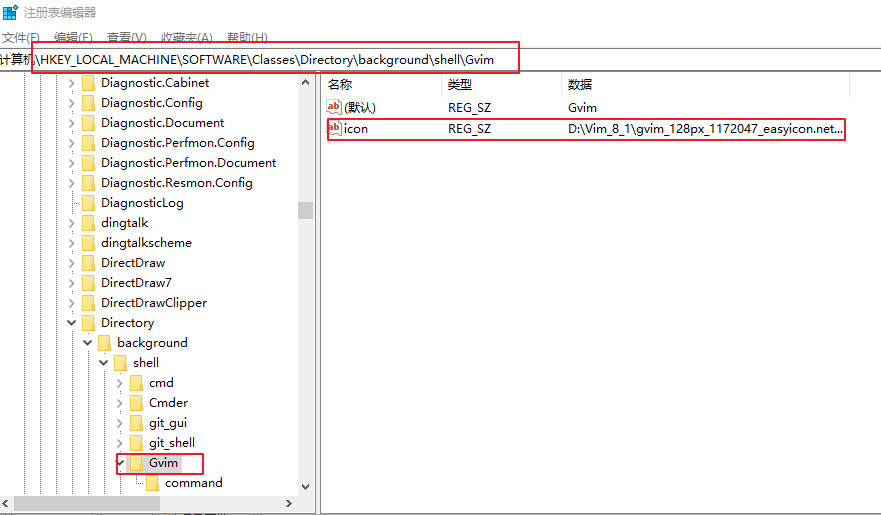
\includegraphics[height=8cm]{add_icon.png}
\caption{添加右键GVIM}
\label{fig:addicon}
\end{figure}

\item 为右键添加图标,点击Rightmenumgr工具,点击注册表编辑器,在该路径下添加相应的图标文件;
\begin{messagebox}
\HKEY_LOCAL_MACHINE\SOFTWARE\Classes\Directory\background\shell\Cmder
\end{messagebox}

\begin{figure}[H]
\centering
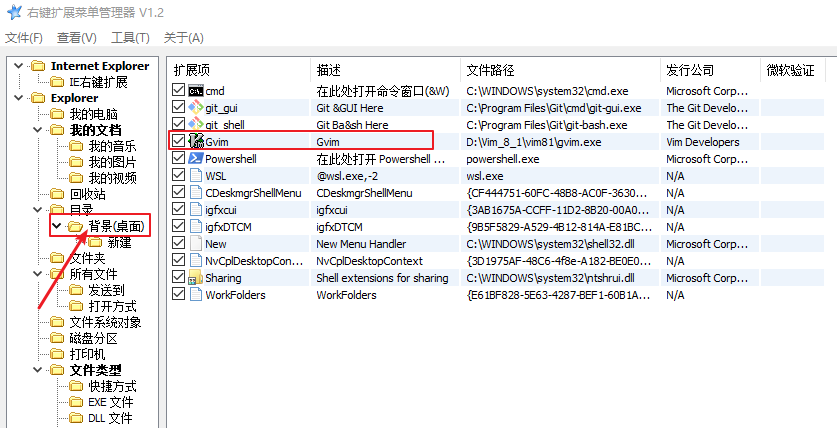
\includegraphics[height=8cm]{rightkey.png}
\caption{添加右键图标}
\label{fig:rightkey}
\end{figure}

\end{itemize}

